% Figure 5 - Early-tag-broadcast timing diagram.
%
% Cycles 0..9 along the x-axis.  Cycle 0 = MULT enters stage 0; the
% early-tag sideband fires.  The dependent RS entry's src_ready is
% registered, so it settles at cycle 1.  The MULT result reaches the CDB at
% cycle 7 and the dependent RS issues that same cycle via the CDB-bypass
% mux.  Without ETB the dependent issue would be deferred to cycle 8.
%
% Implemented as a hand-built TikZ waveform (rectangular pulses) for
% predictable layout independent of tikz-timing version quirks.

\usetikzlibrary{calc, decorations.pathreplacing}

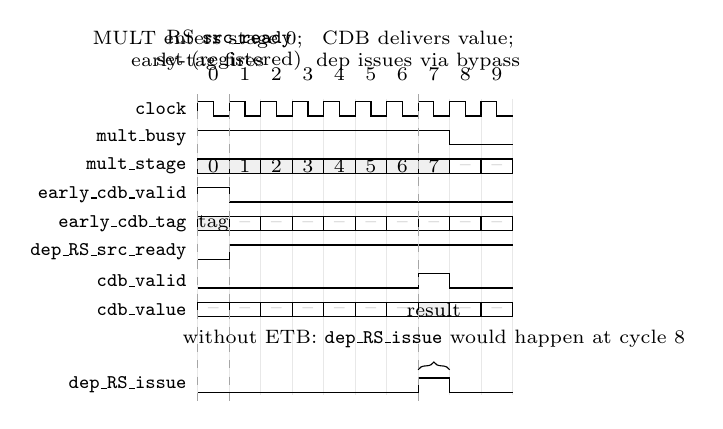
\begin{tikzpicture}[
    font=\scriptsize,
    x=4mm,                  % one TikZ unit = one cycle width
    y=2.6mm,                % one TikZ unit = one row height
    rowlabel/.style = {anchor=east, font=\scriptsize\ttfamily,
                       inner sep=1pt, xshift=-1mm},
    wave/.style     = {line width=0.45pt, line cap=square,
                       line join=miter, color=black},
    guide/.style    = {dashed, gray!70, thin},
    glab/.style     = {font=\scriptsize, align=center, inner sep=1pt}
]

% --- Geometry -----------------------------------------------------------
% Total width spans cycles 0..9 (10 cycles).  Each row is centred at its
% own integer y; the waveform vertical excursion is +/- 0.35.
\def\Ncyc{10}
\def\hi{0.35}
\def\lo{-0.35}

% Row y-positions (top to bottom).  Extra gap before the dep_RS_issue row
% leaves room for the "without ETB" bracket directly above it.
\def\yClk   { 0}
\def\yBusy  {-1.4}
\def\yStg   {-2.8}
\def\yEv    {-4.2}
\def\yEt    {-5.6}
\def\ySr    {-7.0}
\def\yCv    {-8.4}
\def\yCval  {-9.8}
\def\yDi    {-13.5}

% --- Row labels --------------------------------------------------------
\node[rowlabel] at (0, \yClk)  {clock};
\node[rowlabel] at (0, \yBusy) {mult\_busy};
\node[rowlabel] at (0, \yStg)  {mult\_stage};
\node[rowlabel] at (0, \yEv)   {early\_cdb\_valid};
\node[rowlabel] at (0, \yEt)   {early\_cdb\_tag};
\node[rowlabel] at (0, \ySr)   {dep\_RS\_src\_ready};
\node[rowlabel] at (0, \yCv)   {cdb\_valid};
\node[rowlabel] at (0, \yCval) {cdb\_value};
\node[rowlabel] at (0, \yDi)   {dep\_RS\_issue};

% --- Cycle column labels (top) ----------------------------------------
\foreach \c in {0,...,9} {%
    \node[font=\scriptsize, anchor=south]
        at (\c+0.5, \yClk + 0.9) {\c};
}

% --- Light cycle gridlines (very faint) -------------------------------
\foreach \c in {0,1,2,3,4,5,6,7,8,9,10} {%
    \draw[gray!18, line width=0.2pt] (\c, \yClk + 0.5) -- (\c, \yDi - 0.5);
}

% =====================================================================
% clock - square wave: high for first half-cycle, low for second.
% =====================================================================
\draw[wave]
    (0, \yClk + \lo)
    \foreach \c in {0,...,9} {%
        -- (\c,         \yClk + \lo)
        -- (\c,         \yClk + \hi)
        -- (\c + 0.5,   \yClk + \hi)
        -- (\c + 0.5,   \yClk + \lo)
        -- (\c + 1,     \yClk + \lo)
    };

% =====================================================================
% mult_busy - high cycles 0..7, low cycles 8..9.
% =====================================================================
\draw[wave]
    (0, \yBusy + \hi) -- (8, \yBusy + \hi)
    -- (8, \yBusy + \lo) -- (10, \yBusy + \lo);

% =====================================================================
% mult_stage - one labelled cell per cycle for stages 0..7, "--" for 8..9.
% =====================================================================
\foreach \c/\s in {0/0,1/1,2/2,3/3,4/4,5/5,6/6,7/7} {%
    \fill[gray!12] (\c, \yStg + \lo) rectangle (\c+1, \yStg + \hi);
    \draw[wave]    (\c, \yStg + \lo) rectangle (\c+1, \yStg + \hi);
    \node[font=\scriptsize] at (\c+0.5, \yStg) {\s};
}
\foreach \c in {8,9} {%
    \draw[wave] (\c, \yStg + \lo) rectangle (\c+1, \yStg + \hi);
    \node[font=\scriptsize, color=gray!60] at (\c+0.5, \yStg) {--};
}

% =====================================================================
% early_cdb_valid - pulse at cycle 0 only.
% =====================================================================
\draw[wave]
    (0, \yEv + \lo) -- (0, \yEv + \hi)
    -- (1, \yEv + \hi) -- (1, \yEv + \lo)
    -- (10, \yEv + \lo);

% =====================================================================
% early_cdb_tag - "tag" cell at cycle 0, "--" cells for cycles 1..9.
% =====================================================================
\fill[gray!12] (0, \yEt + \lo) rectangle (1, \yEt + \hi);
\draw[wave]    (0, \yEt + \lo) rectangle (1, \yEt + \hi);
\node[font=\scriptsize] at (0.5, \yEt) {tag};
\foreach \c in {1,...,9} {%
    \draw[wave] (\c, \yEt + \lo) rectangle (\c+1, \yEt + \hi);
    \node[font=\scriptsize, color=gray!60] at (\c+0.5, \yEt) {--};
}

% =====================================================================
% dep_RS_src_ready - low cycle 0, high cycles 1..9.
% =====================================================================
\draw[wave]
    (0, \ySr + \lo) -- (1, \ySr + \lo)
    -- (1, \ySr + \hi) -- (10, \ySr + \hi);

% =====================================================================
% cdb_valid - pulse at cycle 7 only.
% =====================================================================
\draw[wave]
    (0, \yCv + \lo) -- (7, \yCv + \lo)
    -- (7, \yCv + \hi) -- (8, \yCv + \hi)
    -- (8, \yCv + \lo) -- (10, \yCv + \lo);

% =====================================================================
% cdb_value - "result" cell at cycle 7, "--" cells elsewhere.
% =====================================================================
\foreach \c in {0,1,2,3,4,5,6,8,9} {%
    \draw[wave] (\c, \yCval + \lo) rectangle (\c+1, \yCval + \hi);
    \node[font=\scriptsize, color=gray!60] at (\c+0.5, \yCval) {--};
}
\fill[gray!12] (7, \yCval + \lo) rectangle (8, \yCval + \hi);
\draw[wave]    (7, \yCval + \lo) rectangle (8, \yCval + \hi);
\node[font=\scriptsize] at (7.5, \yCval) {result};

% =====================================================================
% dep_RS_issue - pulse at cycle 7 only.
% =====================================================================
\draw[wave]
    (0, \yDi + \lo) -- (7, \yDi + \lo)
    -- (7, \yDi + \hi) -- (8, \yDi + \hi)
    -- (8, \yDi + \lo) -- (10, \yDi + \lo);

% =====================================================================
% Vertical guide lines + labels at cycles 0, 1, 7.
% =====================================================================
\foreach \c/\lbl in {%
    0/{MULT enters stage 0;\\early-tag fires},%
    1/{RS \texttt{src\_ready}\\set (registered)},%
    7/{CDB delivers value;\\dep issues via bypass}%
}{
    \draw[guide] (\c, \yClk + 0.7) -- (\c, \yDi + \lo - 0.4);
    \node[glab, anchor=south] at (\c, \yClk + 1.7) {\lbl};
}

% =====================================================================
% Bracket directly above the dep_RS_issue row, spanning the cycle 7..8
% transition to mark the one-cycle ETB benefit.  Path goes left-to-right;
% the default `brace' decoration bulges upward, placing the apex toward
% the label drawn at `above=...'.
% =====================================================================
\draw[decorate, decoration={brace, amplitude=1mm}, thin]
    (7, \yDi + \hi + 0.4) -- (8, \yDi + \hi + 0.4)
    node[midway, above=1.6mm, font=\scriptsize, align=center]
        {without ETB: \texttt{dep\_RS\_issue} would happen at cycle 8};

\end{tikzpicture}
